\usetikzlibrary{automata,positioning}
\tikzstyle{edge} = [draw,thick,->]

  \begin{figure}[h!]
  %\centering
  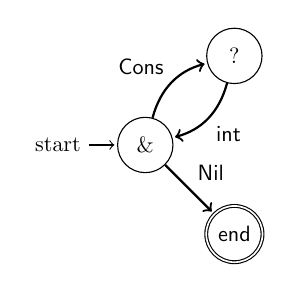
\begin{tikzpicture}[shorten >=1pt,node distance=2cm,on grid,auto, scale=0.8, transform shape]
   \node[state,initial] (choice)   {$\&$}; 
   \node[state] (input) [above right=of choice] {$?$}; 
   \node[state,accepting] (end) [below right=of choice] {\textsf{end}}; 

   \path[edge] (choice) to[bend left] node {\textsf{Cons}} (input);
   \path[edge] (input) to[bend left] node {\textsf{int}} (choice);
   \path[edge] (choice) edge node {\textsf{Nil}} (end);
  \end{tikzpicture}
 %\caption{Autómato finito que representa a serialização de uma lista}
\end{figure}

%%% Local Variables:
%%% mode: latex
%%% TeX-master: "cfst"
%%% End: